\section{Discussion}

The results highlight how the vanilla REINFORCE algorithm struggled to discover a policy that allows the locomotion of the Hopper, achieving a low average reward during training (around $1006$) and displaying low test returns (ranging from $710$ to $1305$).
Practically this means that the agent cannot effectively hop but at most it stays still trying not to fall and at most leap forward and fall. 

As expected, vanilla REINFORCE struggled due to the high variance of full-trajectory Monte Carlo returns, which causes noisy gradient updates, leading to inefficient learning and slow convergence.

Regarding the time needed for training, this was the fastest among the three with a value of $57.6$ minutes, in fact this is primarily driven by episode length,
the Hopper in this case often falls causing the early termination of the episode (the average episode length is $178$), reducing the computational time needed for the learning process.

Introducing a constant baseline of $b{=}20$ had a positive impact on the agent performance. The peak training average reached $1807$ and the test evaluations showed that the best-performing seed achieved a mean test return of
$2444$.

This means that the agent was able to learn a policy that allowed it to effectively hop and move forward for a longer period of time.
The baseline is subtracted from the Monte Carlo return to reduce the variance of the gradient estimates. This reduces the amount of noise in the gradient updates, leading to a more stable and efficient learning process. 
This also improved the average episode length, which increased from 178 to 215, meaning that the agent was able to stay alive for longer periods of time. 

This is also reflected in the average training time that was significantly higher with a value of $70.3$ minutes, proving that the agent
was not falling for a longer period of time.

While a constant baseline ($b=20$) reduced variance and improved performance over vanilla REINFORCE, it applies a global correction that is identical across all states. Actor-Critic further improved stability by using a state-dependent baseline $V(s)$, which adapts to the local structure of the value function, providing a much more effective variance reduction at each step.

The results obtained in the first part demonstrate that the proposed Actor-Critic framework successfully learned a locomotion policy for the Hopper environment.
Indeed, as Figure~\ref{fig:experiments_reward} shows, the Hopper initially discovered balancing and survival behaviours in the first 40,000 episodes, resulting in relatively
low rewards and short episode lengths.
Subsequently, a sharp performance improvement occurred between 40,000 and 55,000 episodes, corresponding to an increase of both reward
and episode duration, suggesting that the agent discovered forward locomotion for the first time.
After this transition phase, training entered a high-performance regime in which average rewards approached 2000 and individual episodes
occasionally exceeded a reward of 3000.
These results demonstrate that the agent discovered effective hopping.
Nevertheless, training did not fully converge to a stable hopping policy: significant reward variance remained throughout the final stages of training, 
indicating that the learned policy was still too exploratory and stochastic, causing it to be unable to reproduce its best behaviors consistently.

This result represents a substantial improvement compared to earlier Actor-Critic implementations tested during development.
Preliminary versions frequently converged to a "lazy" policy in which the Hopper stood still, which can mathematically occur
due to the Hopper maximizing only the survival component of the reward function.

Standing actions were continuously selected as they tended to achiev high positive advantages, meaning these
actions consistently produced outcomes that were better than the critic’s expectations.
On the other hand, jumping actions continuously turned out to be worse than the critic’s expectations.
This occurred due to the initial usage of the TD(0) target, in which only the immediate subsequent
state was considered, so jumping actions always led to immediate worse states, making them less appealing to a
short-sighted critic and discouraging their exploration.
Therefore, the short-sighted critic reinforced actions that led to immediate better states: standing,
which continued to return a positive reward thanks to the survival component of the reward function, forcing the
Hopper to adopt a reward-exploiting local optimum behavior.

Although such behaviour produced relatively stable trajectories, it prevented the discovery of effective locomotion and resulted in poor returns.
The introduction of GAE, a sigma floor together with advantage normalization, a learned exploration variance, a triggered learning-rate decay mechanism
significantly improved exploration and enabled the policy to free itself from the local optimum, eventually discovering hopping.

The final model's behavioral instability seems to be supported by the critic-loss spikes, which, however, 
should not necessarily be interpreted as training failure.
These spikes are not necessarily indicative of unstable training as reinforcement-learning targets
continuously change together with the current policy, therefore when the actor discovers substantially better trajectories,
previously learned value estimates become obsolete and inaccurate, generating large temporal-difference errors and
consequently large critic-loss spikes. This reasoning proves that the critic loss irregularity is caused by its own outdated
estimates and it trying to keep up with the new updated policy, demonstrating that an unsteady critic loss is quite inevitable
as it is caused by the Reinforcement Learning intrinsic dynamicity.

This interpretation is supported by the fact that critic spikes often coincide with newly discovered high-reward behaviors,
such as the discovery of hopping.

In contrast, actor updates remained remarkably stable throughout training, as advantage normalization successfully bounded
policy updates and prevented gradient explosions despite the highly non-stationary learning process.

Despite these improvements, the final policy still exhibits substantial variability and has not fully converged. Future work
could investigate additional stabilization techniques like TRPO or PPO which exploits trust region and clipped policy
updates (Schulman et al., 2017).

Furthermore, more advanced actor-critic methods for continuous control, such as DDPG and TD3, could be explored,
exploiting double-critic architectures and delayed policy updates, to potentially reduce value-estimation errors
and improve training stability (Fujimoto et al., 2018).


\begin{figure}[htbp]
    \centering
    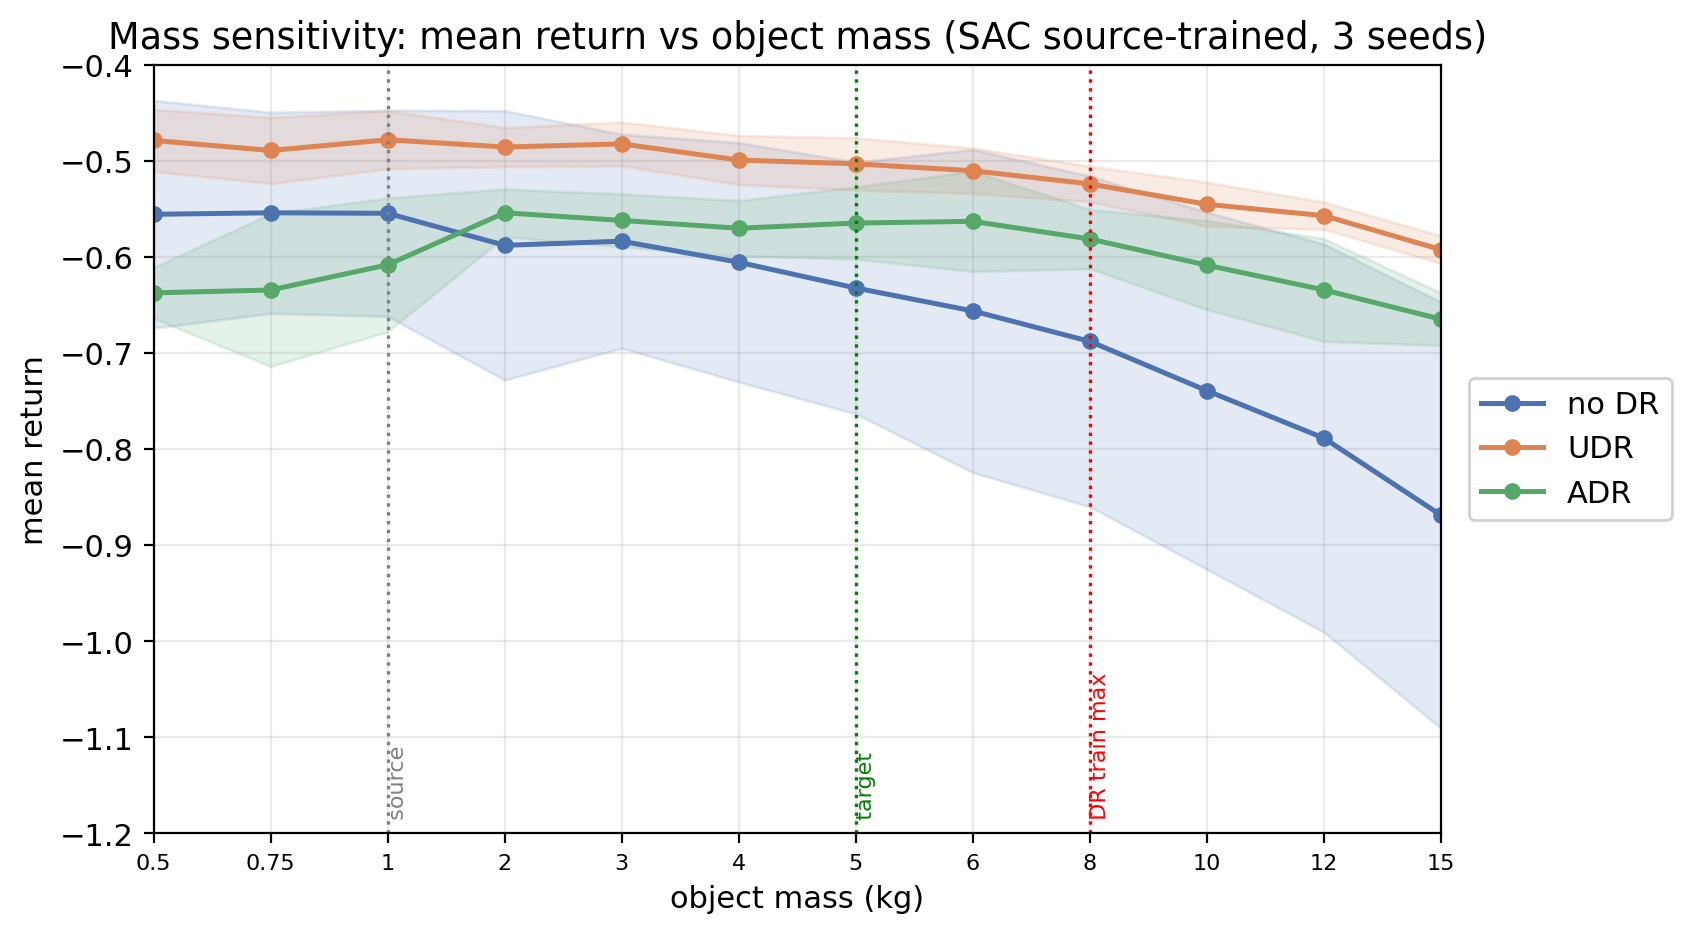
\includegraphics[width=\columnwidth]{imgs/sensitivity_return.png}
    \caption{Mass-sensitivity analysis.}
    \label{fig:sensitivity}
\end{figure}